\documentclass[a4paper,10pt]{article}

\usepackage{graphicx}
\usepackage[utf8]{inputenc}
\usepackage[T1]{fontenc}
\usepackage{wrapfig}

\usepackage{hyperref}
\setlength{\parindent}{10pt}
\setlength{\parskip}{1.5mm}
\usepackage{geometry}
\geometry{margin=1.25cm}
\addtolength{\textheight}{-1.5cm}
\setlength{\headheight}{32pt}

\usepackage{amsfonts, amstext, color,
	ifthen, fancybox, multirow, fancyhdr, pgf, tikz,%
	colortbl, array, tabularx
}

\definecolor{bgcode}{rgb}{0.95,0.95,0.95}

\usepackage{url}

\usepackage[french]{babel}
\selectlanguage{french}

%partie concernant la gestion des entêtes
\usepackage{fancyhdr}
\pagestyle{fancy}
\usepackage{lastpage}
\renewcommand\headrulewidth{1pt}
\fancyhead[L]{Interface Homme-Machine Android}
\fancyhead[R]{Université de Poitiers}
\renewcommand\footrulewidth{1pt}
\fancyfoot[L]{Département d'Informatique}
\fancyfoot[C]{\textbf{\thepage/\pageref{LastPage}}}
\fancyfoot[R]{année 2021-2022}
%fin

\usepackage{enumitem}

\usepackage{listings}

\usepackage{version}
\usepackage{tcolorbox}

\newcounter{Exercice}
\newcommand{\Exercice}[1]{\refstepcounter{Exercice}%
	\ \vspace{0mm} \\ \hspace{0.8cm}%
	\noindent \hspace*{0.5cm} {\bf Question \theExercice :} #1 \vspace{-13mm} \\ %
	\subparagraph*{}%
}

\lstset{language=Caml,basicstyle=\normalsize\tt,keywordstyle=\ttfamily\bfseries\underbar,%
	commentstyle=\normalsize, extendedchars=true, fontadjust=true, columns = flexible, flexiblecolumns=true,
	linewidth=.975\linewidth, backgroundcolor=\color{bgcode}, frame=tlrb, xleftmargin=1cm}

\lstnewenvironment{ocamlcode}
{\lstset{language=Caml,basicstyle=\normalsize\tt,keywordstyle=\ttfamily\bfseries\underbar,%
		commentstyle=\normalsize, extendedchars=true, fontadjust=true, columns = flexible, flexiblecolumns=true,
		linewidth=.975\linewidth, backgroundcolor=\color{bgcode}, frame=tlrb, xleftmargin=1cm,
		literate={à}{{\`a}}1 {è}{{\`e}}1 {é}{{\'e}}1 {ê}{{\^e}}1,
	}}%, framexleftmargin=5mm,frame=box}}
{}

\lstnewenvironment{fsharp}
{\lstset{language=Caml,basicstyle=\normalsize\tt,keywordstyle=\ttfamily\bfseries\underbar,%
		commentstyle=\normalsize, extendedchars=true, fontadjust=true, columns = flexible, flexiblecolumns=true,
		linewidth=.975\linewidth, backgroundcolor=\color{bgcode}, frame=tlrb, xleftmargin=1cm,
		literate={à}{{\`a}}1 {è}{{\`e}}1 {é}{{\'e}}1 {ê}{{\^e}}1 {ç}{{\c c}}1,
}}%, framexleftmargin=5mm,frame=box}}
{}

\lstnewenvironment{javasansbord}
{\lstset{language=Java,basicstyle=\normalsize\tt,keywordstyle=\ttfamily\bfseries\underbar,%
		commentstyle=\normalsize, extendedchars=true, fontadjust=true, columns = flexible, flexiblecolumns=true,
		linewidth=.975\linewidth,frame=,backgroundcolor=,xleftmargin=0cm,
		literate={à}{{\`a}}1 {è}{{\`e}}1 {é}{{\'e}}1 {ê}{{\^e}}1 {ç}{{\c c}}1,
}}%, framexleftmargin=5mm,frame=box}}
{}

\lstnewenvironment{java}
{\lstset{language=Java,basicstyle=\normalsize\tt,keywordstyle=\ttfamily\bfseries\underbar,%
		commentstyle=\normalsize, extendedchars=true, fontadjust=true, columns = flexible, flexiblecolumns=true,
		linewidth=.975\linewidth, backgroundcolor=\color{bgcode}, frame=tlrb, xleftmargin=1cm,
		literate={à}{{\`a}}1 {è}{{\`e}}1 {é}{{\'e}}1 {ê}{{\^e}}1 {ç}{{\c c}}1,
}}%, framexleftmargin=5mm,frame=box}}
{}

\newboolean{versionenseignant}
%%%%%%%%%%%%%%%%%%%%%%%%%%%%%%%%%%%%%%%%%%%%%%%%%%%%%%%%%%%%%%%%%%%%%%%%%%%%%%%%%%%%%%%%%%%%%%%%%%%%%%%%
%__     __            _
%\ \   / /__ _ __ ___(_) ___  _ __
% \ \ / / _ \ '__/ __| |/ _ \| '_ \
%  \ V /  __/ |  \__ \ | (_) | | | |
%   \_/ \___|_|  |___/_|\___/|_| |_|
% _____                _                         _
%| ____|_ __  ___  ___(_) __ _ _ __   __ _ _ __ | |_
%|  _| | '_ \/ __|/ _ \ |/ _` | '_ \ / _` | '_ \| __|
%| |___| | | \__ \  __/ | (_| | | | | (_| | | | | |_
%|_____|_| |_|___/\___|_|\__, |_| |_|\__,_|_| |_|\__|
%                        |___/ 
%% modifiez le booleen ci-dessous pour generer la version enseignant ou etudiant
%% ===> true = version enseignant
%% ===> false = version etudiant
\setboolean{versionenseignant}{false}
%%%%%%%%%%%%%%%%%%%%%%%%%%%%%%%%%%%%%%%%%%%%%%%%%%%%%%%%%%%%%%%%%%%%%%%%%%%%%%%%%%%%%%%%%%%%%%%%%%%%%%%%
% \includeversion{ensnote}
%\excludeversion{ensnote}
\ifthenelse{\boolean{versionenseignant}}{\includeversion{ensnote}}{\excludeversion{ensnote}}

\tcbuselibrary{breakable}


\newenvironment{solution}%
{\begin{tcolorbox}[breakable,colback=red!5!white,colframe=red!75!black,title=Solution]}%
{\end{tcolorbox}}

%\tcblower

\newenvironment{info}%
{\begin{tcolorbox}[breakable,colback=green!5!white,colframe=green!75!black,title=Information]}%
{\end{tcolorbox}}


\newenvironment{attention}%
{\begin{tcolorbox}[breakable,colback=green!25!white,colframe=red!55!black,title=Attention]}%
{\end{tcolorbox}}


\newenvironment{boxcode}%
{\begin{tcolorbox}[breakable,colback=gray!5!white,colframe=black]}%
	{\end{tcolorbox}}
	
	
\begin{document}
	


\title{\vspace*{-1cm}Réalisation d'un widget complexe}
\author{\vspace*{-1.5cm}Interface Homme-Machine: Unity
\begin{ensnote}
	(Version enseignant)
\end{ensnote}
}
\date{\vspace*{-1.5cm}version 1}
\maketitle
\thispagestyle{fancy}


%\begin{attention}
%	Le sujet ce fait en deux étapes. Avec une proposition notée de votre interface au bout de 2h (si vous avez fini avant la \textit{deadline} rien ne vous empêche de continuer)!
%	
%	N'oubliez pas d'utiliser les bons réflexes de tout développeur:
%	\begin{itemize}
%		\item Le système de log très bien fait sous Android
%		\item Le mode débogue qui vous permet de voir les valeurs des variables pendant 
%	\end{itemize}
%\end{attention}

\section{Réalisation d'un spinner latéral}




Une application a besoin d'un spinner dont les boutons pour défiler les valeurs entières sont situées sur les cotés du composant. Ce widget se nommera \texttt{LatSpinner} (pour \textit{lateral spinner}), et propose une plage de valeur valide encoder sous forme d'un code couleur, c'est à dire que les valeurs non-valide peuvent aussi être affichée mais l'utilisateur a un retour visuel sous forme de couleur dans notre exemple qui insiste sur ce point. Vous devez donc réaliser un tel widget et vous devez respecter les consignes suivantes:
\begin{itemize}
	\item Vous ne devez pas utiliser de ressources extérieur à Unity de base.
	\item Vous devez respecter la version du cours sous peine d'avoir zéro à cet exercice.
	\item Les textes de notre widget doivent s'adapter à leur taille.
	\item Les textes doivent être aligner horizontalement et verticalement.
	\item Vous devez avoir un code visuel clair pour indiquer si la valeur en cours est valide ou non.
	\item Le widget doit être interactif, et lorsqu'on clique sur les boutons, la valeur doit évoluer selon un pas (step) choisi par l'utilisateur de votre widget.
	\item Votre widget doit avoir des propriétés paramétrables directement dans Unity (en particulier celles que devra manipuler votre utilisateur)
	\item Votre widget doit s'adapter aux redimensionnements de ce dernier.
	\item La valeur numérique ne doit pas être modifiable au clavier, mais copiable pour le coller sur une application extérieure.
\end{itemize}

Vous remettez un zip (j'ai bien dit ZIP et pas autre chose sinon 0) de projet, qui illustre plusieurs \texttt{LatSpinner} avec des valeurs adéquats et un fichier unitypackage qui reprend l'export uniquement du \texttt{LatSpinner} en vue d'une utilisation future.

\begin{center}
	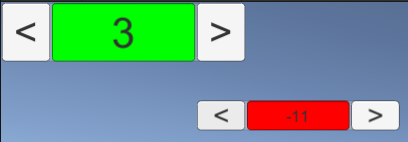
\includegraphics[width=0.7\linewidth]{LatSpinner}
\end{center}

\end{document}